% ------------------------------------------------------------------------
% Relatório - Física II - UFPR (modelo abntex2)
% Itens em vermelho, no formato [ ... ], são pendências: procurem por \pend
% e removam todos antes de entregar.
% ------------------------------------------------------------------------
\documentclass[
12pt,			% tamanho da fonte
openany,		% capítulos começam em qualquer página (sem folhas em branco)
oneside,		% para leitura digital/impressão só de um lado
a4paper,		% tamanho do papel
sumario=tradicional,
chapter=TITLE,
section=TITLE,
subsection=Title,
brazil,			% idioma principal do documento
]{abntex2}

% ---
% Pacotes fundamentais
% ---
\usepackage[T1]{fontenc}
\usepackage{helvet}
\renewcommand{\familydefault}{\sfdefault}
\usepackage[utf8]{inputenc}
\usepackage{indentfirst}
\usepackage{xcolor}
\usepackage{graphicx}
\usepackage{microtype}
\usepackage{siunitx}
\usepackage{booktabs}
\sisetup{output-decimal-marker={,}, range-phrase={~a~}, range-units=single, group-digits=false}

% Pendências visíveis (em vermelho) para não esquecer nada antes da entrega
\newcommand{\pend}[1]{\textcolor{red}{\textit{[#1]}}}

% ---
% Pacote de citações padrão ABNT
% ---
\usepackage[alf,no-abnt-option-file,abnt-citacoes-mistas]{abntex2cite}

% ---
% Dados do relatório
% ---
\titulo{Temperatura de superfície no campus Politécnico: comparação entre fragmento florestal e áreas antropizadas com imagem Landsat}
\autor{Nome do Aluno 1 \\ Nome do Aluno 2 \\ Nome do Aluno 3}
\local{Curitiba}
\data{\the\year}

% ---
% Espaçamentos e fontes
% ---
\setlength{\parindent}{1.3cm}
\setlength{\parskip}{0.2cm}

\renewcommand{\ABNTEXchapterfontsize}{\normalsize}
\renewcommand{\ABNTEXsectionfontsize}{\normalsize}
\renewcommand{\chaptitlefont}{\normalfont\bfseries\normalsize}
\renewcommand{\chapnumfont}{\normalfont\bfseries\normalsize}

\begin{document}
	
	\selectlanguage{brazil}
	\frenchspacing
	
	% ----------------------------------------------------------
	% ELEMENTOS PRÉ-TEXTUAIS
	% ----------------------------------------------------------
	
	% ---
	% Folha de rosto
	% ---
	\thispagestyle{empty}
	\begin{center}
		\textbf{UNIVERSIDADE FEDERAL DO PARANÁ}
		
		\vspace{2.5cm}
		\uppercase {
			Ana Luiza Cislinsky \\
			Lucas de Oliveira Ferreira \\
			Milena Silva
		}
		\vspace{2.5cm}

		
		\vspace{3cm}
		\uppercase{Temperatura de superfície no campus Politécnico: comparação entre fragmento florestal e áreas antropizadas com imagem Landsat}
	\end{center}
	
	\vspace{1cm}
	\noindent\hspace{0.45\textwidth}
	\begin{minipage}{0.50\textwidth}
		Relatório apresentado como requisito parcial para aprovação na disciplina de Física II, como acompanhamento do seminário sobre termodinâmica e extensão universitária.
		
		\bigskip
		Professora: Dr\textsuperscript{a} Lucieli Rossi
	\end{minipage}
	
	\vfill
	\begin{center}
		\textbf{CURITIBA}\\
		\the\year
	\end{center}
	\newpage
	
	% ---
	% Resumo
	% ---
	\setlength{\absparsep}{18pt}
	\begin{resumo}
		
		A cobertura do solo influencia o comportamento térmico das superfícies, uma vez que diferentes materiais e tipos de vegetação apresentam características distintas de absorção, armazenamento e transferência de energia. Nesse contexto, este trabalho teve como objetivo comparar a temperatura de superfície de fragmentos florestais e áreas antropizadas no Campus Politécnico da Universidade Federal do Paraná (UFPR), em Curitiba, relacionando as diferenças observadas aos princípios da termodinâmica. Para isso, foi utilizada uma imagem do satélite Landsat 8-9, referente a 12 de abril de 2026, para estimar a temperatura de superfície das duas classes de cobertura. Também foram utilizados dados de temperatura e umidade relativa do ar, obtidos na estação meteorológica do Instituto Nacional de Meteorologia (INMET) para estimar a evapotranspiração de referência por meio do modelo Moretti-Jerszurki-Silva. Os resultados indicaram temperatura média de 26,61 °C nos fragmentos florestais e 30,48 °C nas áreas antropizadas, representando uma diferença de 3,87 °C. Essa diferença pode ser interpretada a partir do balanço de energia da superfície, considerando a contribuição da evapotranspiração e do sombreamento proporcionado pela vegetação para a dissipação e distribuição da energia recebida. Os resultados demonstram como os conceitos da termodinâmica podem ser aplicados à compreensão das diferenças térmicas entre ambientes com distintas características de cobertura do solo.
		
		\noindent
		\textbf{Palavras-chave}:  Termodinâmica; temperatura de superfície; cobertura do solo; evapotranspiração; Landsat.
	\end{resumo}
	
	% ---
	% Sumário
	% ---
	\pdfbookmark[0]{\contentsname}{toc}
	\tableofcontents*
	\cleardoublepage
	
	% ----------------------------------------------------------
	% ELEMENTOS TEXTUAIS
	% ----------------------------------------------------------
	\textual
	\pagestyle{simple}
	
	\chapter{Introdução}
	
	A lei da condução térmica demonstra que diferentes materiais possuem capacidades distintas de conduzir o calor \cite{halliday}. Sob essa visão, a distribuição da temperatura nas superfícies terrestres não acontece de forma homogênea, uma vez que materiais distintos interagem de diferentes maneiras com a energia. Portanto, áreas urbanas tendem a alterar o microclima, uma vez que as construções impermeáveis das cidades retêm muito calor \cite{ribeiro2016clima}. Em contraste, ambientes com cobertura vegetal armazenam menos calor, oferecem sombra e autorregulam-se por meio da evapotranspiração, gerando um maior conforto térmico. 

	A partir dos princípios da termodinâmica conseguimos analisar, comparar e compreender essas diferenças. Ao compararmos as temperaturas em diferentes ambientes conseguimos compreender o compartimento térmico divergente. Assim, este trabalho teve como objetivo comparar a temperatura de superfície de fragmentos florestais e áreas antropizadas no Campus Politécnico da Universidade Federal do Paraná (UFPR), em Curitiba, utilizando dados do satélite Landsat. Adicionalmente, buscou-se relacionar as diferenças observadas aos processos de transferência de calor e ao balanço de energia da superfície, discutindo a contribuição dos conceitos da termodinâmica para a compreensão das condições térmicas do ambiente.

	
	\chapter{Fundamentação teórica}
	
	\section{Temperatura, calor e equilíbrio térmico}
	
	A temperatura determina o sentido da transferência espontânea de calor entre corpos: o calor, que é energia em trânsito por causa de uma diferença de temperatura, flui do corpo mais quente para o mais frio até que se atinja o equilíbrio térmico. Em cálculos termodinâmicos, a temperatura $T$ deve ser expressa em escala absoluta, em \si{\kelvin}, que se relaciona com a temperatura Celsius $T_C$ por $T_C = T - 273{,}15$ \cite{halliday}.
	
	\section{Formas de transferência de calor}\label{sec:transferencia}
	
	O calor se transfere de três maneiras \cite{halliday}. Na condução, a energia passa de uma região a outra de um material por colisões entre suas partículas, como o calor que penetra no solo. A taxa de transferência de energia por uma placa de área $A$ e espessura $L$, com faces às temperaturas $T_Q$ e $T_F$ ($T_Q > T_F$), é
	
		\begin{equation}
		P_{\mathrm{cond}} = k \, A \, \frac{T_Q - T_F}{L},
	\end{equation}
	
	\noindent em que:
	\begin{alineas}
		\item $P_{\mathrm{cond}}$ é a taxa de transferência de energia por condução, em \si{\watt};
		\item $k$ é a condutividade térmica do material;
		\item $A$ é a área da placa;
		\item $L$ é a espessura da placa;
		\item $T_Q$ e $T_F$ são as temperaturas das faces quente e fria, com $T_Q > T_F$.
	\end{alineas}
	
	Na convecção, a energia é carregada pelo movimento de um fluido, como o ar aquecido junto ao chão que sobe e é substituído por ar mais frio. Na radiação, a energia é transportada por ondas eletromagnéticas e não precisa de meio material, como a energia que o Sol envia à Terra \cite{atmos}.
	
	Todo corpo emite radiação térmica. A taxa com que um corpo real emite energia é dada pela lei de Stefan-Boltzmann \cite{halliday}:
	
	\begin{equation}
		P_{\mathrm{rad}} = \sigma \, \varepsilon \, A \, T^{4},
	\end{equation}
	
	\noindent em que:
	\begin{alineas}
		\item $P_{\mathrm{rad}}$ é a taxa de emissão de energia por radiação, em \si{\watt};
		\item $\sigma = \SI{5.6704e-8}{\watt\per\metre\squared\per\kelvin\tothe{4}}$ é a constante de Stefan-Boltzmann;
		\item $\varepsilon$ é a emissividade da superfície;
		\item $A$ é a área da superfície emissora;
		\item $T$ é a temperatura absoluta da superfície.
	\end{alineas}
	
	O comprimento de onda de máxima emissão é dado pela lei de Wien:
	
	\begin{equation}
		\lambda_{\max} \, T = b,
	\end{equation}
	
	\noindent em que:
	\begin{alineas}
		\item $\lambda_{\max}$ é o comprimento de onda de máxima emissão;
		\item $T$ é a temperatura absoluta da superfície;
		\item $b \approx \SI{2.898e-3}{\metre\kelvin}$ é a constante de deslocamento de Wien.
	\end{alineas}
	
	Para superfícies à temperatura ambiente, $\lambda_{\max}$ fica em torno de \SI{10}{\micro\metre}, na faixa do infravermelho termal. Por isso o sensor termal do Landsat, que opera nessa faixa, permite estimar a temperatura de superfície a partir da radiação medida.
	
	
	\section{Calor sensível e calor latente}
	
		
	Quando o calor absorvido por um corpo muda sua temperatura, tem-se \cite{halliday}:
	
	\begin{equation}
		Q = c \, m \, (T_f - T_i),
	\end{equation}
	
	\noindent em que:
	\begin{alineas}
		\item $Q$ é o calor absorvido pelo corpo;
		\item $c$ é o calor específico do material;
		\item $m$ é a massa do corpo;
		\item $T_i$ e $T_f$ são as temperaturas inicial e final do corpo.
	\end{alineas}
	
	Esse é o calor que a meteorologia chama de sensível \cite{atmos}, pois se manifesta como variação de temperatura. Quando há mudança de fase, ao contrário, a energia absorvida ou liberada não altera a temperatura do material. Para a vaporização de uma massa de água, tem-se \cite{halliday}:
	
	\begin{equation}
		Q = L_V \, m,
	\end{equation}
	
	\noindent em que:
	\begin{alineas}
		\item $Q$ é o calor absorvido na vaporização;
		\item $L_V$ é o calor de vaporização (também chamado de calor latente de vaporização);
		\item $m$ é a massa de água vaporizada.
	\end{alineas}
	
	Na evapotranspiração, parte da energia recebida pela vegetação é gasta nessa mudança de fase, o que limita o aumento de temperatura das folhas e do solo sombreado \cite{yang2023}.
	
	
	\section{Balanço de energia da superfície}
	
	A primeira lei da termodinâmica, $\Delta E_{\mathrm{int}} = Q - W$, expressa a conservação de energia \cite{halliday}. Em uma superfície muito fina, a variação de energia interna é desprezível ($\Delta E_{\mathrm{int}} \approx 0$), de modo que a energia que chega é igual à que sai. Isso resulta no balanço de energia, em que o saldo de radiação recebido se distribui entre aquecimento do ar, evaporação e aquecimento do solo:
	
		
	\begin{equation}
		R_n = H + LE + G, \label{eq:balanco}
	\end{equation}
	
	\noindent em que:
	\begin{alineas}
		\item $R_n$ é o saldo de radiação (radiação absorvida menos a emitida);
		\item $H$ é o fluxo de calor sensível, que aquece o ar por convecção;
		\item $LE$ é o fluxo de calor latente, associado à evaporação ou à transpiração;
		\item $G$ é o fluxo de calor conduzido ao solo.
	\end{alineas}
	
	Cada termo é uma taxa de transferência de energia por unidade de área, em \si{\watt\per\metre\squared}, como $P_{\mathrm{cond}}/A$ e $P_{\mathrm{rad}}/A$ da Seção~\ref{sec:transferencia}; em particular, $LE = L_V \, (\Delta m/\Delta t)/A$ para uma massa $\Delta m$ de água evaporada no intervalo $\Delta t$. Os símbolos $R_n$, $H$, $LE$ e $G$ são os usuais em meteorologia \cite{atmos}. Termos menores, como o calor armazenado na vegetação, são desprezados.
	
	Como $H$ e $G$ só levam energia da superfície ao ar e ao solo se ela estiver mais quente que eles, uma superfície que dissipa a maior parte de $R_n$ por $LE$ tende a ficar mais fria que outra que a dissipa principalmente por $H$ e $G$.
	
	\chapter{Métodos}
	
	\section{Área de estudo}
	
	O estudo foi realizado no campus Politécnico (Centro Politécnico) da Universidade Federal do Paraná, em Curitiba. Delimitaram-se duas classes de cobertura: fragmento florestal, formado pelas duas áreas de floresta nativa existentes no campus e tratadas em conjunto, e as áreas antropizadas, correspondentes ao restante do campus.
	
	\section{Dados de satélite}
	
	Foi utilizada imagem do satélite Landsat 8-9, sensor OLI/TIRS, Coleção 2, Nível 2, obtida no portal do USGS \cite{usgs}. A imagem é de 12/04/2026, com passagem às 10h17 (horário de Brasília). Utilizou-se o produto de temperatura de superfície ST\_B10, derivado da banda termal 10 (\SIrange{10.6}{11.2}{\micro\metre}). O produto é distribuído com pixels de \SI{30}{\metre}. A data foi escolhida por apresentar céu sem nuvens sobre o campus. 
	Os polígonos foram delimitados manualmente, de forma digital, por fotointerpretação de imagens de satélite do Google, carregadas como camada no QGIS \cite{google}.
	
	\section{Dados da estação meteorológica}
	
	Os valores de temperatura do ar e de umidade relativa vieram da estação meteorológica automática do Instituto Nacional de Meteorologia (INMET), em Curitiba (código A807), situada no campus Politécnico, a \SI{923}{\metre} de altitude \cite{inmet2026}. Os dados são fornecidos em UTC e foram convertidos para o horário local. Para a comparação, usou-se o registro das 10h locais (13h UTC) do mesmo dia da imagem, o mais próximo da passagem do satélite, com temperatura de \SI{22.0}{\celsius} e umidade relativa de 57\%.
	
	Todas as áreas análisadas ficam todas dentro de um raio de aproximadamente  \SI{1,1}{\kilo\metre} da estação.
	
	\subsection{Temperatura de superfície}
	
	Os valores digitais foram convertidos em Kelvin pelos fatores de escala fornecidos nos metadados da cena, e em seguida, em graus Celsius: 
	
	\begin{equation}
		T = \num{0.00341802} \, \mathrm{DN} + \num{149.0}, \qquad T_C = T - 273{,}15.
	\end{equation}
	
	O produto já faz correções atmosféricas e de emissividade, de modo que não foi necessário tratamento além da conversão.
	
	Para comparar a superfície com o ar, calculou-se a diferença:
	
		\begin{equation}
		\Delta T = T_{\text{superfície}} - T_{\text{ar}},
	\end{equation}
	
	\noindent em que $T_{\text{ar}}$ é a temperatura do ar registrada pela estação.
	
	\section{Evapotranspiração de referência}
	
	A evapotranspiração de referência ($ET_0$) é a taxa com que uma superfície padronizada, sem falta de água, perde água por evaporação e transpiração; ela mede a demanda evaporativa da atmosfera \cite{fao}. Foi estimada pelo modelo Moretti-Jerszurki-Silva (MJS), que parte do potencial hídrico do ar, $\Psi_{\mathrm{ar}}$, calculado apenas com a temperatura e a umidade relativa do ar \cite{dossantos2021}:
	
	\begin{equation}
		\Psi_{\mathrm{ar}} = \frac{R \, T}{V_m} \, \ln\left(\frac{\mathrm{UR}}{100}\right),
	\end{equation}
	
	\begin{alineas}
		\item $R = \SI{8.314}{\joule\per\mole\per\kelvin}$ é a constante dos gases;
		\item $T$ é a temperatura absoluta do ar;
		\item $V_m = \SI{18e-6}{\cubic\metre\per\mole}$ é o volume molar parcial da água;
		\item $\mathrm{UR}$ é a umidade relativa, em \%.
	\end{alineas}
	
	Com essas unidades, $\Psi_{\mathrm{ar}}$ resulta em pascal e é negativo: quanto mais seco o ar, mais negativo o valor e maior a demanda por evaporação. O cálculo de $\Psi_{\mathrm{ar}}$ se baseia na primeira e na segunda lei da termodinâmica \cite{dossantos2021}.
	
	A evapotranspiração é então obtida por uma relação linear com $\Psi_{\mathrm{ar}}$:
	
	\begin{equation}
		ET_0 = \alpha + \beta \, \Psi_{\mathrm{ar}},
	\end{equation}
	
	\noindent em que $\alpha = \SI{-0.024}{\milli\metre\per\hour}$ e $\beta = \SI{-3.595e-9}{\milli\metre\per\hour\per\pascal}$ são os coeficientes obtidos para Curitiba na calibração horária do modelo em relação ao método de Penman-Monteith padrão, com coeficiente de correlação $r = 0{,}66$ \cite{dossantos2021}. Os cálculos do modelo foram feitos no software R.
	
	Para expressar a demanda evaporativa como fluxo de energia, converte-se $ET_0$ em calor latente. Assim:
	
	\begin{equation}
		LE_0 \approx 680 \, ET_0,
	\end{equation}
	
	com $LE_0$ em \si{\watt\per\metre\squared} e $ET_0$ em \si{\milli\metre\per\hour}.
	
	\chapter{Resultados}
	
	A Figura~\ref{fig:mapa} apresenta o mapa de temperatura de superfície da área de estudo. As maiores temperaturas (acima de \SI{31.82}{\celsius}) aparecem em manchas no nordeste, no oeste e no sudoeste do campus, e as menores (até \SI{26.55}{\celsius}), no norte e no centro-sul, onde estão as duas áreas de floresta nativa. Em geral, as áreas antropizadas concentram as temperaturas mais elevadas, enquanto o fragmento florestal apresenta valores menores.
	
	\begin{figure}[htb]
		\centering
		\caption{Temperatura de superfície no campus Politécnico (imagem Landsat de 12/04/2026, 10h17).}
		\fbox{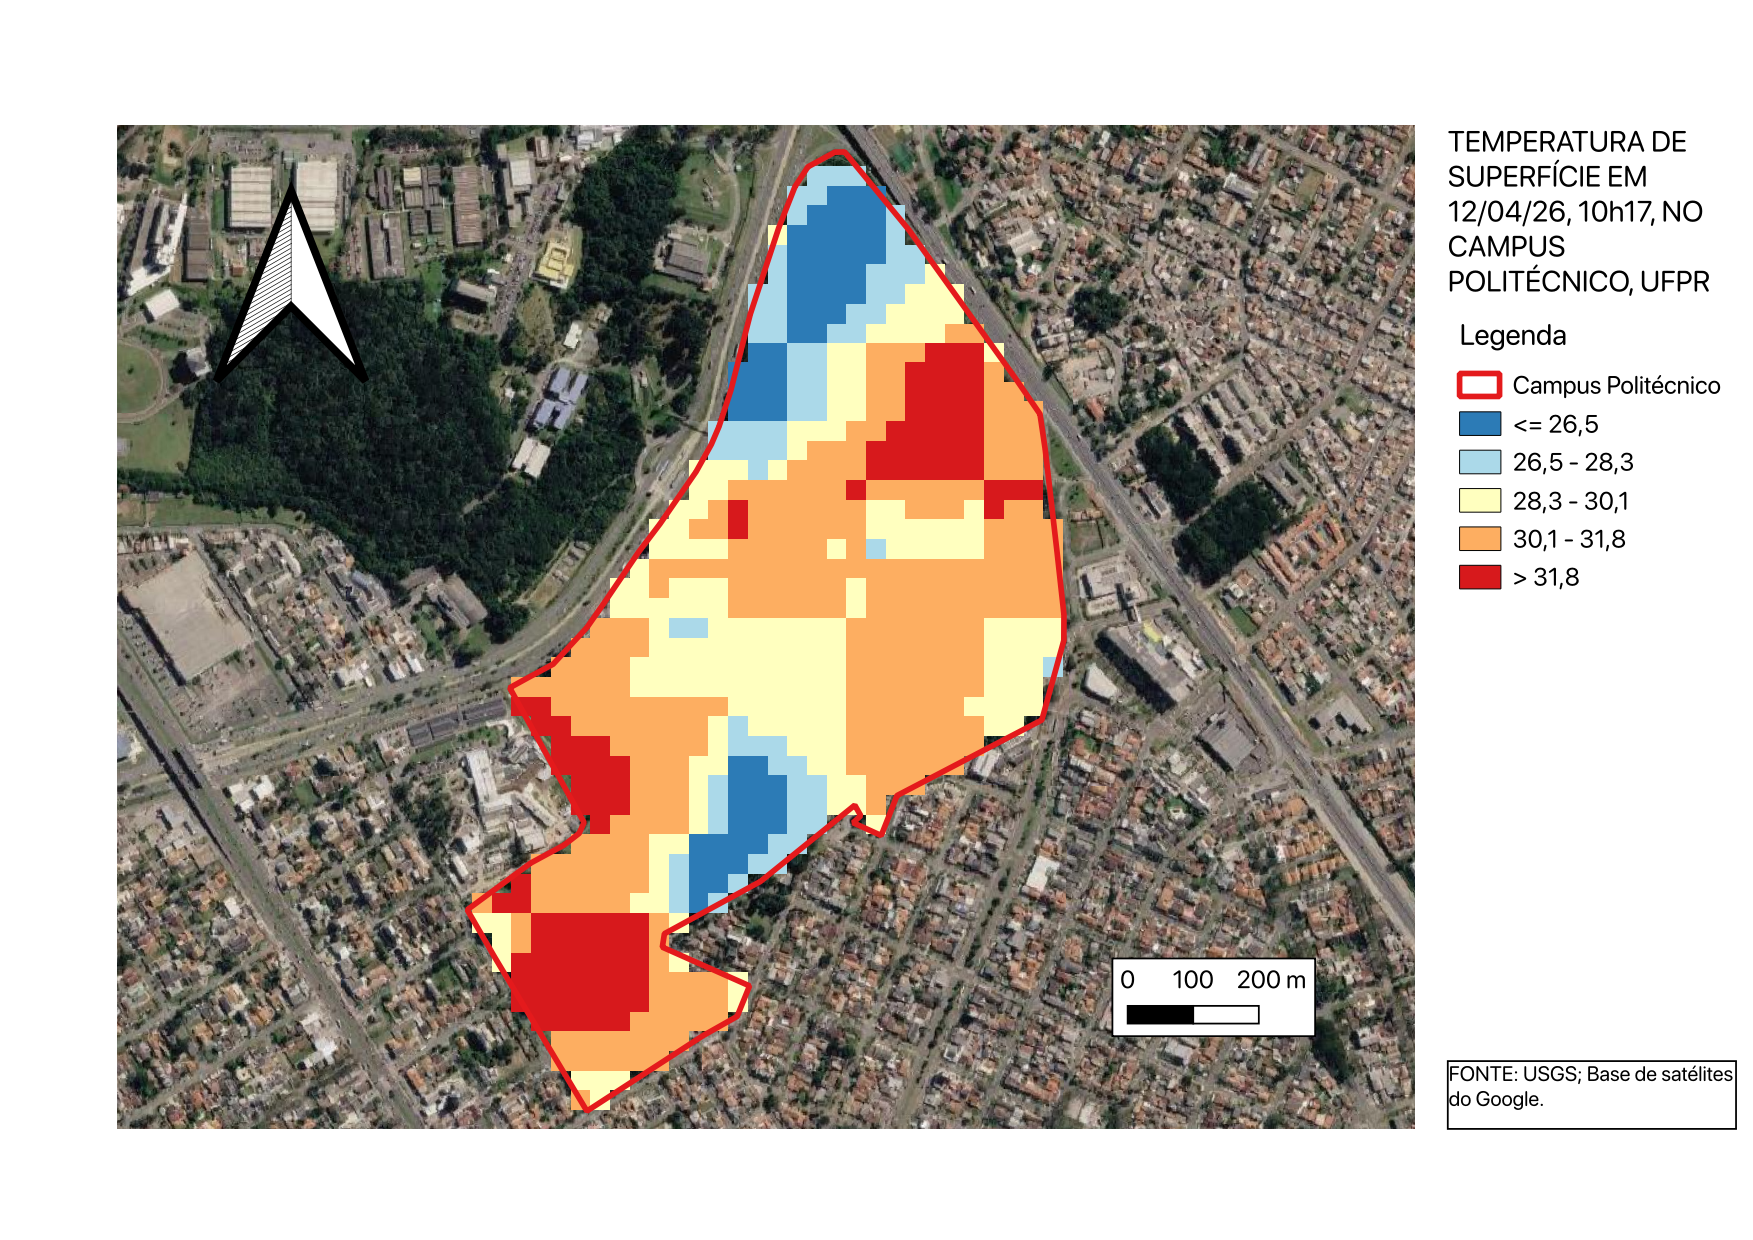
\includegraphics[width=0.75\textwidth]{img/ilhas.png}}
		\label{fig:mapa}
		\small \fonte{Elaborado pelos autores (2026), sobre imagem de satélite do Google (\citeyear{google}) e dados do USGS (\citeyear{usgs}).}
	\end{figure}
	
	A Tabela~\ref{tab:resultados} apresenta a temperatura média de superfície de cada classe. A média das áreas antropizadas supera a do fragmento florestal em \SI{3.87}{\celsius}.
	
	\begin{table}[htb]
		\centering
		\caption{Temperatura média de superfície por classe de cobertura.}
		\label{tab:resultados}
		\begin{tabular}{lc}
			\toprule
			Classe & Temperatura média (\si{\celsius}) \\
			\midrule
			Fragmento florestal & 26,61 \\
			Áreas antropizadas & 30,48 \\
			\midrule
			Diferença (antropizadas menos fragmento) & 3,87 \\
			\bottomrule
		\end{tabular}
		\fonte{Elaborado pelos autores (2026) com dados do USGS(\citeyear{usgs}).}
	\end{table}
	
	A Tabela~\ref{tab:estacao} compara as temperaturas de superfície de cada classe com a temperatura do ar registrada pela estação no horário mais próximo da passagem do satélite.
	
	\begin{table}[htb]
		\centering
		\caption{Temperatura do ar a \SI{2}{\metre} (registro das 10h) e temperatura média de superfície por classe (passagem do satélite às 10h17).}
		\label{tab:estacao}
		\begin{tabular}{lcc}
			\toprule
			Medida & Temperatura (\si{\celsius}) & $\Delta T$ em relação ao ar (\si{\celsius}) \\
			\midrule
			Ar a \SI{2}{\metre} (estação INMET) & 22,0 & -- \\
			\midrule
			Superfície: fragmento florestal & 26,61 & 4,61 \\
			Superfície: áreas antropizadas & 30,48 & 8,48 \\
			\bottomrule
		\end{tabular}
		\fonte{Elaborado pelos autores com dados do USGS(\citeyear{usgs}) e do INMET(\citeyear{inmet2026}).}
	\end{table}
	
	A Figura~\ref{fig:estacao} mostra a evolução horária da temperatura do ar e da umidade relativa no dia da imagem. Na passagem do satélite, o ar estava em aquecimento e secagem rápidos. Interpolando linearmente entre os registros das 10h e das 11h, os valores às 10h17 seriam \SI{22.28}{\celsius} e 55,3\%, diferenças de \SI{0.28}{\celsius} e 1,7 ponto percentual em relação ao registro das 10h, que foi o usado nos cálculos.
	
	\begin{figure}[htb]
		\centering
		\caption{Temperatura do ar e umidade relativa em 12/04/2026, com a passagem do Landsat às 10h17 (13h17 UTC).}
		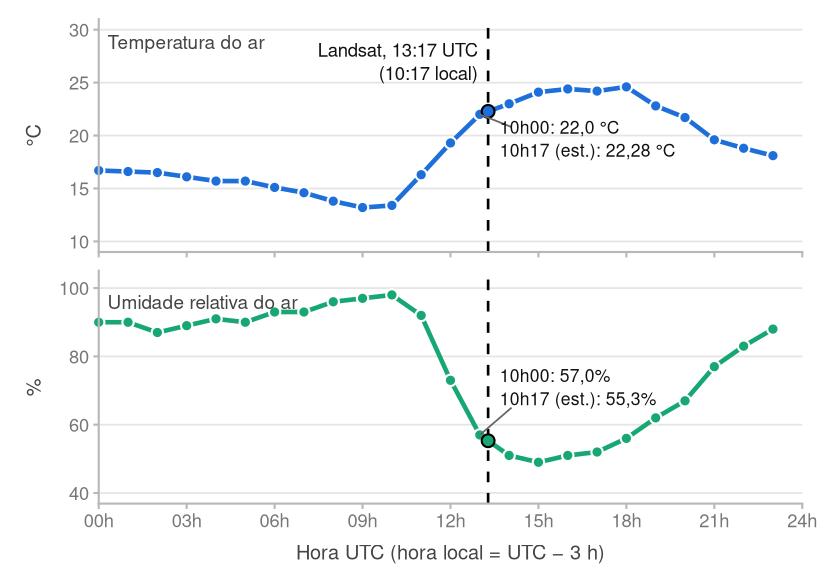
\includegraphics[width=0.75\textwidth]{img/graph.png}
		\label{fig:estacao}
		\small \fonte{Elaborado pelos autores (2026) com dados do INMET (\citeyear{inmet2026}).}
	\end{figure}
	
	Para o registro das 10h, com temperatura do ar de \SI{22.0}{\celsius} e umidade relativa de 57\%, o potencial hídrico do ar é de aproximadamente \SI{-7.66e7}{\pascal} (cerca de \SI{-76.6}{\mega\pascal}). A evapotranspiração de referência estimada pelo modelo MJS é de cerca de \SI{0.25}{\milli\metre\per\hour}, o que corresponde a aproximadamente \SI{171}{\watt\per\metre\squared} de calor latente.
	
	\chapter{Discussão e limitações}
	
	O contraste observado entre as classes de uso e cobertura do solo pode ser interpretado a partir do balanço de energia da superfície. A principal diferença entre essas classes está na partição da energia disponível entre os diferentes fluxos. Nas áreas antropizadas, predominam superfícies impermeáveis e com menor disponibilidade de água, o que limita a energia dissipada pelo processo de evaporação. Dessa forma, uma parcela maior do saldo de radiação tende a ser distribuída entre o fluxo de calor sensível ($H$) e o fluxo de calor no solo ($G$). Nos fragmentos florestais, por sua vez, a evapotranspiração representa uma parcela importante do consumo energético, na forma de calor latente ($LE$), enquanto o sombreamento proporcionado pelo dossel tende a reduzir o fluxo de calor para o solo. Ressalta-se, entretanto, que esses fluxos não foram medidos diretamente neste estudo.
	
	Ambas as classes apresentaram temperaturas de superfície superiores à temperatura do ar, embora em magnitudes distintas. As áreas antropizadas registraram uma diferença de $8{,}48\,^{\circ}\mathrm{C}$ em relação ao ar, enquanto nos fragmentos florestais essa diferença foi de $4{,}61\,^{\circ}\mathrm{C}$. Esse comportamento é compatível com as condições observadas no período da manhã, quando a radiação solar promove o aquecimento das superfícies, que transferem parte dessa energia para a atmosfera por meio de convecção. Em uma aproximação simplificada, o fluxo de calor sensível ($H$) tende a aumentar com a diferença de temperatura entre a superfície e o ar, o que sugere um maior potencial de aquecimento da camada de ar próxima à superfície nas áreas antropizadas. Adicionalmente, a energia armazenada no solo e nos materiais construtivos pode ser liberada posteriormente, contribuindo para a persistência de temperaturas elevadas e para o resfriamento mais lento dessas áreas.
	
	O valor estimado de $LE_0$, de aproximadamente $171\,\mathrm{W\,m^{-2}}$, representa a demanda evaporativa da atmosfera nas condições meteorológicas do horário analisado, e não a energia efetivamente dissipada pelos fragmentos florestais na forma de calor latente. Esta última depende também da disponibilidade hídrica do solo, das condições da vegetação e da resistência à transferência de vapor d'água.
	
	\section{Limitações}
	
	Os resultados devem ser interpretados considerando algumas limitações metodológicas:
	
	\begin{enumerate}
		\item A análise foi realizada a partir de uma única imagem de satélite não permitindo avaliar a variabilidade diária ou sazonal da temperatura de superfície;
		
		\item O produto de temperatura de superfície apresenta incertezas inerentes ao processo de estimativa. Além disso, a resolução espacial pode resultar em pixels mistos, especialmente nas bordas dos fragmentos florestais;
		
		\item Os dados de temperatura do ar foram obtidos em uma única estação meteorológica, não representando as condições micrometeorológicas.
		
		\item Existe uma diferença de aproximadamente 17 minutos entre o horário de registro dos dados meteorológicos e o momento da passagem do satélite, o que pode introduzir diferenças nas condições atmosféricas utilizadas na análise.
		
		\item A estimativa de $ET_0$ foi realizada por meio de um método empírico, cujas limitações podem influenciar os resultados em escala horária. Além disso, conforme discutido por \citeonline{dossantos2021}, o método tende a subestimar os valores de evapotranspiração nessa escala.
	\end{enumerate}
	
	\chapter{Termodinâmica e extensão universitária}
	\label{cap:extensao}
	
	A Constituição Federal determina que as universidades obedeçam ao princípio da indissociabilidade entre ensino, pesquisa e extensão \cite{cf1988}. Na extensão, o conhecimento produzido e ensinado na universidade chega à sociedade e, no sentido inverso, os problemas e as perguntas da comunidade voltam à universidade como temas de estudo.
	
	O Projeto Nimbus é um exemplo próximo. Vinculado ao Laboratório de Climatologia (LaboClima) da UFPR, tem como finalidade mostrar a importância da observação meteorológica para a sociedade. Para isso, organiza visitas guiadas ao campus Politécnico, em que estudantes de Curitiba e região metropolitana conhecem uma estação meteorológica e participam de atividades educativas e lúdicas conduzidas por monitores. Desde 2022, o projeto também realiza aulas, palestras e oficinas em escolas \cite{nimbus}.
	
	Os resultados deste relatório podem ser traduzidos em uma atividade curta para esse público. A proposta, ainda não aplicada, tem três passos: (i) medir, com um termômetro infravermelho, a temperatura de superfície da grama, da sombra de uma árvore, do concreto e do asfalto, e compará-la com a temperatura do ar registrada pela estação; (ii) mostrar o mapa de satélite do campus e pedir que os participantes identifiquem onde estão as áreas mais quentes e por quê; (iii) discutir o que a comunidade pode fazer para reduzir o calor urbano, como ampliar a arborização e manter áreas permeáveis e vegetadas. A atividade usa as ideias da fundamentação teórica sem equações: a vegetação ajuda a refrescar o ambiente porque a água que evapora consome energia, e materiais escuros e impermeáveis absorvem e guardam calor. O termômetro infravermelho também depende da emissividade do material (Seção~\ref{sec:transferencia}), o que permite discutir como a medida é feita.
	
	% ----------------------------------------------------------
	% ELEMENTOS PÓS-TEXTUAIS
	% ----------------------------------------------------------
	\postextual
	\pagebreak
	
	\bibliography{referencias}
	
\end{document}